\documentclass{article}
\usepackage{fullpage}
\usepackage[utf8]{inputenc}
\usepackage{graphicx}
\usepackage[ngerman]{babel}
\usepackage{hyperref}
\usepackage{tabularx}
\usepackage{attachfile}
\usepackage{pdfpages}
\usepackage{siunitx}
\usepackage{caption} \captionsetup[table]{skip=10pt}

\title{Physikalisches Grundpraktikum 1 für Bachelor in Gruppen:\\Akustik (AKU)}
\author{Technische Universität München\\\\Leon Heiß, Paul Hildebrandt \\
Kurs 5, Gruppe 7, Team 19}
\date{24. Mai 2022}
\renewcommand*\contentsname{Inhaltsverzeichnis}

\renewcommand{\abstract}[1]{{ \noident {\bf\\Einleitung \\} #1 }}

\begin{document}

\maketitle

% normale Einleitung will bei mir nicht kompilieren...
\large
\begin{center}
\textbf{Abstract}\\
\normalsize
\medskip
Ziel des Akustik Versuches ist es, die Schallgeschwindigkeit in Luft und Festkörpern zu bestimmen.
Hierbei wird zunächst die Laufgeschwindigkeit des Schalls in drei verschiedenen Stäben ermittelt.
Zudem führt man eine Laufzeitmessung in der Luft durch und im letzten Teilversuch werden stehende
Wellen in einem Rohr näher betrachtet.

\end{center}
\normalsize

\tableofcontents

\section{Grundlagen}
\subsection{Allgemeines zu Wellen}
Übt man eine Kraft auf eine elastisches Medium aus oder anders gesagt, verschiebt es aus seiner Gleichgewichtslage, so erfährt das Medium eine in seine Ruhelage zurücktreibende Kraft.
Wegen der  Elastizität des Materials, genauer genommen aufgrund der Bindungskräfte zwischen den Atomen, wird diese  Störung auf benachbarte Bereiche übertragen und als Welle im Medium fortgeleitet. Das Medium als Ganzes bewegt sich dabei nicht mit der Welle voran; nur die einzelnen Elemente, auf mikroskopischer Ebene des Mediums, schwingen in einem sehr  beschränkten  Bereich  um  die  Gleichgewichtslage. 
Die Schwingungsrichtung der enstandenen Welle kann entweder senkrecht zur Ausbreitungsrichtung der Welle (\textbf{Transversalwelle}) oder parallel (\textbf{Longitudinalwelle}) dazu stehen.
\begin{figure}[hbt!]
\centering
\includegraphics[scale=0.18]{ausbreitungsrichtung.png}
\caption{Transversale (a) und longitudinale (b) Schwingungen, aus Versuchsanleitung \cite{1} .}
\end{figure}
\subsection{Wichtige Kenngrößen}
Um eine Welle mathematisch beschreiben zu können, braucht es verschiedene charakteristische Kenngrößen, wie die Wellenlänge $\lambda$, welche für den Abstand zwischen zwei Wellenbergen steht und die Schwingungsdauer $T$, welche die Zeitdauer für ein volle Schwingung bis zur Wiederholung des Vorgangs beschreibt. \\Des Weiteren stellt die Amplitude $A$ die maximale Auslenkung der harmonischen Schwingung da und $\omega = \frac{2 \pi}{T} $ die Kreisfrequenz. Zudem wird die Beziehung $k=\frac{2\pi}{\lambda}$ als Wellenzahl und $\phi$ als Phase der Welle bezeichnet.\\
Mit diesen Größen kann man nun die allgemeine Wellengleichung aufstellen:
\begin{equation}
a(t,x)= A \cdot \cos(\omega \cdot t - k \cdot x + \phi)
\end{equation}
Um die Geschwindigkeit der sich ausbreitenden Welle zu bestimmen, betrachtet man die Verschiebung der Welle um eine Wellenlänge pro Schwingunsdauer. Daraus lässt sich der Schwingungszustand (Phase $\phi$) der Welle messen, die Geschwindigkeit dieser Phase nennt sich die Phasengeschwindigkeit und ist gegeben durch 
\begin{equation}
v = \frac{\lambda}{T} = \frac{\omega}{k} = f \cdot \lambda .
\end{equation}
Ein weiteres wichtiges Maß für die Beschreibung von Wellen ist die Frequenz $f = \frac{1}{T}$, welche die Anzahl der Schwingungen pro Zeiteinheit beschreibt.
\subsection{Schallgeschwindigkeit in verschiedenen Medien}
Die Ausbreitungsgeschwindigkeit in elastischen Medien hängt primär von der Dichte $\rho$ des und der Kopplung zwischen den Atomen des Mediums ab.
\subsubsection{Feskörper}
In Festköpern treten sowohl longitudinale als auch transversale Wellen auf, jedoch werden in diesem Versuch nur longitudinale Schwingungen betrachtet.
Longitudinale Schallwellen bewegen sich in langen Stäben (mit im Vergleich zur Wellenlänge kleinen Durchmessern) mit der Geschwindigkeit
\begin{equation}
v_{FK, longitudinal} = \sqrt{\frac{E}{\rho}},
\end{equation}
wobei $\rho$ hier die Dichte des Mediums und $E$ das Elastizitätsmodul ist.
\subsubsection{Gase}
Anstatt des Elastizitätsmodul $E$ verwendet man in Gasen und Flüssigkeiten das Kompressionsmodul K. Die Phasengeschwindigkeit für longitudinale Wellen in Gasen ist somit
\begin{equation}
    v_{Fl,Gas} = \sqrt{\frac{K}{\rho}}
\end{equation}
Bei idealen Gasen gilt für adiabatische Zustandsänderung, also für Übergangsprozesse bei denen keine Wärmeenergie mit der Umgebung ausgetauscht wird, der folgende Zusammenhang zwischen Druck und Volumen
\begin{equation}
    p \cdot V^\kappa = const. \quad \textrm{mit} \quad \kappa = \frac{c_{p}}{c_V}
\end{equation}
$\kappa$ ist hierbei der Adiabatenkoeffizient, welcher den Quotient der spezifischen Wärmekapazitäten des Gases bei konstantem Druck bzw. Volumen beschreibt. Diese Zusammenhänge werden später dafür genutzt, die Schallgeschwindigkeit in einem idealen Gas zu bestimmen.
Alternativ lässt sich Gleichung 4 bei idealen Gasen auch zu:
\begin{equation}
    v_{Gas} = \sqrt{\kappa \frac{p}{\rho}} = \sqrt{\kappa \frac{RT}{M}}
\end{equation}
umformen, wobei $p$ der Druck, $R$ die ideale Gaskonstante, $T$ die Temperatur, $M$ die molare Masse und $\kappa$ der Adiabatenkoeffizient ist. Zu beachten ist jedoch, dass $v_{gas}$ von der Wurzel der absoluten Temperatur abhängt:
\begin{equation}
    v_{Gas}(T)= v_{Gas}(T_0) \cdot \sqrt{\frac{T}{T_0}}.
\end{equation}
\subsubsection{Stehende Wellen}
Als stehende Wellen bezeichnet man solche, deren Amplitude an bestimmten stellen stets null ist. Sie können durch Überlagerung gegenläufiger Wellen mit gleicher Frequenz und Amplitude sowie fester Phase erzeugt werden. Betrachtet man zwei Wellen
\begin{equation}
    w_1(t,x) = A \cdot cos(\omega \cdot t - k \cdot x)
\end{equation}
\begin{equation}
    w_2(t,x) = A \cdot cos(\omega \cdot t + k \cdot x + \phi)
\end{equation}
so lässt sich $w_1 + w_2$ mithilfe der Additionstheoreme umformen zu
\begin{equation}
    w_{Interferenz}(t,x) = 2\cdot A \cdot cos(\omega \cdot t + \frac{\phi}{2}) \cdot cos(k \cdot x + \frac{\phi}{2})
\end{equation}
mit einem Cosinus-Term, der ausschließlich ortsabhängig ist und einem Cosinus-Term, der ausschließlich zeitabhängig ist. Dadurch entstehen Punkte, an denen die Amplitude stets null ist und dazwischen oszillierende Wellenbäuche. \cite{1}

\section{Laufzeitmessung im Festkörper}
\subsection{Versuchsaufbau}
Um die longitudinale Schallgeschwindigkeit in einem Festkörper zu bestimmen, platziert man einen Stab auf einem Schalldetektor, welcher an ein Oszilloskop angeschlossen ist, und erzeugt am oberen Ende des Stabs einen Schallimpuls.
Der ausgelöste Schallimpuls durchläuft den Stab und erzeugt ein Signal am Sensor. Da aber nun der Schallimpuls am unteren Ende des Rohres reflektiert wird und nochmalig den Stab durchläuft, wird ein weiteres Signal am Sensor erzeugt. Aus der Zeitdifferenz und der doppelten Stablänge lässt sich dann die Schallgeschwindigkeit ermitteln.
\begin{figure}[hbt!]
\centering
\includegraphics[scale=0.2]{aufbau_festkörper.png}
\caption{ a) Aufbau und b) Oszilloskop Ausgabe zur Laufzeitmessung, aus Versuchsanleitung \cite{1}.}
\end{figure}
\subsection{Auswertung}
Um die unterschiedlichen Schallgeschwindigkeiten in den jeweiligen Materialien zu bestimmen, nutzt man aus, dass der Schallimpuls am unteren Ende des Stabes ein Signal am Detektor auslöst, reflektiert, nochmalig den Stab durchläuft und ein weiteres Signal am Detektor auslöst. Daraus lässt sich schließen, dass die Ausbreitungsgeschwindigkeit im Inneren des Stabes folgende Beziehung hat:

\begin{equation}
v_{FK} = \frac{2 \cdot l}{t}
\end{equation}
wobei $l$ die jeweilige Stablänge und $t$ die doppelte Laufzeit der Welle durch den Stab ist. Hierbei wurde angenommen, dass nur longitudinale und keine transversalen Wellen auftreten.\\
Um nun die Elastizitätsmodule der Stäbe zu bestimmen, stellen wir Gleichung 3 nach $E$ um:
\begin{equation}
    E = v^2 \cdot \rho
\end{equation}
Die von uns bestimmten numerischen Werte sind in Tabelle 1 aufgetragen.

\begin{table}[hbt!]
\caption{Schallgeschwindigkeit und Elastizitätsmodul der drei verschiedenen Stäbe}
\centering
\begin{tabular}{|l|l|l|l|l|l|l|}
\hline
\rule{0pt}{10pt}
Material & Stablänge l [m] & Laufzeit t [$\SI{}{\micro\meter}$] &  $v_{FK}$ [m/s] & $v_{FK,Lit}$ [m/s]&  $E$ [GPa] & $E_{Lit}$ [GPa] \\ \hline
Kupfer & 1,500 $\pm$ 0,002 & 778,4 $\pm$ 20,0  & 3854,1 $\pm$ 99,1 & 3810 &  132,94 $\pm$ 0,81 &   125              \\ \hline
Eisen & 1,490  $\pm$ 0,002 & 602,4 $\pm$ 20,0  & 4970,1 $\pm$ 163,2 & 4994 & 192,68 $\pm$ 2,51  &   210            \\ \hline
PVC & 1,020  $\pm$ 0,001 & 1225,6 $\pm$ 40,0 & 1669,4 $\pm$ 54,3 & 1950 &  3,90 $\pm$ 0,56 &   3,3            \\ \hline
\end{tabular}
\end{table}
Die ermittelten Werte für die Schallgeschwindigkeit und das Elastizitätsmodul stimmen größtenteils innerhalb der Unsicherheiten mit Literaturewerten \cite{2} \cite{3} \cite{5} überein.

\subsection{Fehlerrechnung}
In diesem Teilversuch sind zwei wichtige Unsicherheiten zu beachten.
Zunächst hat der Meterstab, mit dem jeweils die Länge $l$ der einzelnen Stäbe bestimmt wurde, eine gewisse Fertigungsgenauigkeit, welcher in der Versuchsanleitung \cite{1} als
\begin{equation}
u(l)= a + b \cdot L
\end{equation}
gegeben ist. Hierbei ist $a=0,6$ mm, $b=0,4$ mm/m und $L$ sei die auf den nächsten vollen Meter aufgerundete gemessene Länge.\\
Des Weiteren ist uns eine mögliche Fehlerquelle beim Kupferrohr aufgefallen, welche durch eine Einkerbung (2) und (3) in Abb. 3 an den jeweiligen Enden des Stabes vorhanden ist. An dieser können Schallwellen reflektiert werden, die sich dann mit den Schallwellen, die an (1) reflektiert werden, überlagern. Da diese Fehlerquelle jedoch nicht trivial zu berücksichtigen ist und die Messergebnisse vermutlich nicht allzu sehr beeinträchtigt, entschieden wir uns, sie zu vernachlässigen.
\begin{figure}
\centering
\includegraphics[scale=0.3]{Stäbe_Abschluss.png}
\caption{Vergleich Eisenrohr zu Kupferrohr: Mögliche Fehlerquelle durch Reflektion an Einkerbung im Kupferrohr }
\end{figure}
Die zweite wichtige Unsicherheit ist die der Zeit $t$ am Oszilloskop. Da die Genauigkeit des Oszilloskops auf der Zeitachse typischerweise nur $0,01 \%$ \cite{1}  beträgt, ist der begrenzende Faktor die Ablesegenauigkeit bzw. Einstellungsgenauigkeit des Cursors (bei uns $\SI{20}{\micro\meter}$).

Mithilfe der Gaußschen Fehlerfortpflanzung lassen sich jetzt die Geschwindigkeitsunsicherheiten folgendermaßen berechnen:

\begin{equation}
u(v_i)=  v_i \cdot \sqrt{\bigg(\frac{u(l_i)}{l_i}\bigg)^2 + \bigg(\frac{u(t_i)}{t_i}\bigg)^2}.
\end{equation}
In weiterer Folge erhält man die Unsicherheiten $u(E)$ der Elastizitätsmodule, indem man wiederum die Gaußsche Fehlerfortpflanzung auf die bereits hergeleitete Gleichung 7 anwendet:
\begin{equation}
u(E) = E \cdot \sqrt{\bigg(\frac{2u(v_i)}{v_i}\bigg)^2 + \bigg(\frac{u(\rho_i)}{\rho_i}\bigg)^2}.
\end{equation}
Sowohl $\rho$ als auch $u(\rho)$ stammen aus der der Versuchsanleitung \cite{1}.

\section{Laufzeitmessung in der Luft}
\subsection{Versuchsaufbau}
Mithilfe von zwei Mikrofonen, die an ein Oszilloskop angeschlossen sind, wird in diesem Teilversuch die Schallgeschwindigkeit in Luft bestimmt. Die Mikrofone werden in variablem Abstand $d$ auf einer Achse in die selbe Richtung orientiert angeordnet. Anschließend erzeugt man auf der selben Achse in ca. 1 Meter Entfernung des ersten Mikrofons mittels zweier Metallkugeln einen Schallimpuls. Am Oszilloskop lässt sich nun eine Zeitdifferenz $\Delta t$ zwischen der Aufnahme des Schallimpulses durch das erste und der des zweiten Mikrofons ablesen. Dieser Vorgang wird nun für verschiedene Abstände $d$ wiederholt.
\begin{figure}[hbt!]
\centering
\includegraphics[scale=0.2]{aufbau_luft.png}
\caption{a) Aufbau und b) Oszilloskop Ausgabe zur Laufzeitmessung in der Luft, aus Versuchsanleitung \cite{1}.}
\end{figure}

\subsection{Auswertung}
Um die Schallgeschwindigkeit aus der Laufzeitmessung zwischen den beiden Mikrofonen zu bestimmen, tragen wir die Wegdifferenz $d$ gegen die Zeit $t$ auf.
Anschließend legen wir eine Ausgleichsgerade durch unsere Messpunkte und berechnen die Geradensteigung. 
Die von uns bestimmte Geradensteigung entspricht nun der gesuchten Schallgeschwindigkeit, man erhält $v = (340,64 \pm 19,76)$ m/s. Treffen tut die Geradengleichung den Ursprung nicht, da dies bedeuten würde, dass beide Mikrofone auf der exakt gleichen Position wären. Verglichen mit dem Literaturwert von $v=346$ m/s \cite{2}, stellt dies eine Abweichung von 1,5 \% da.


\begin{figure}[hbt!]
\centering
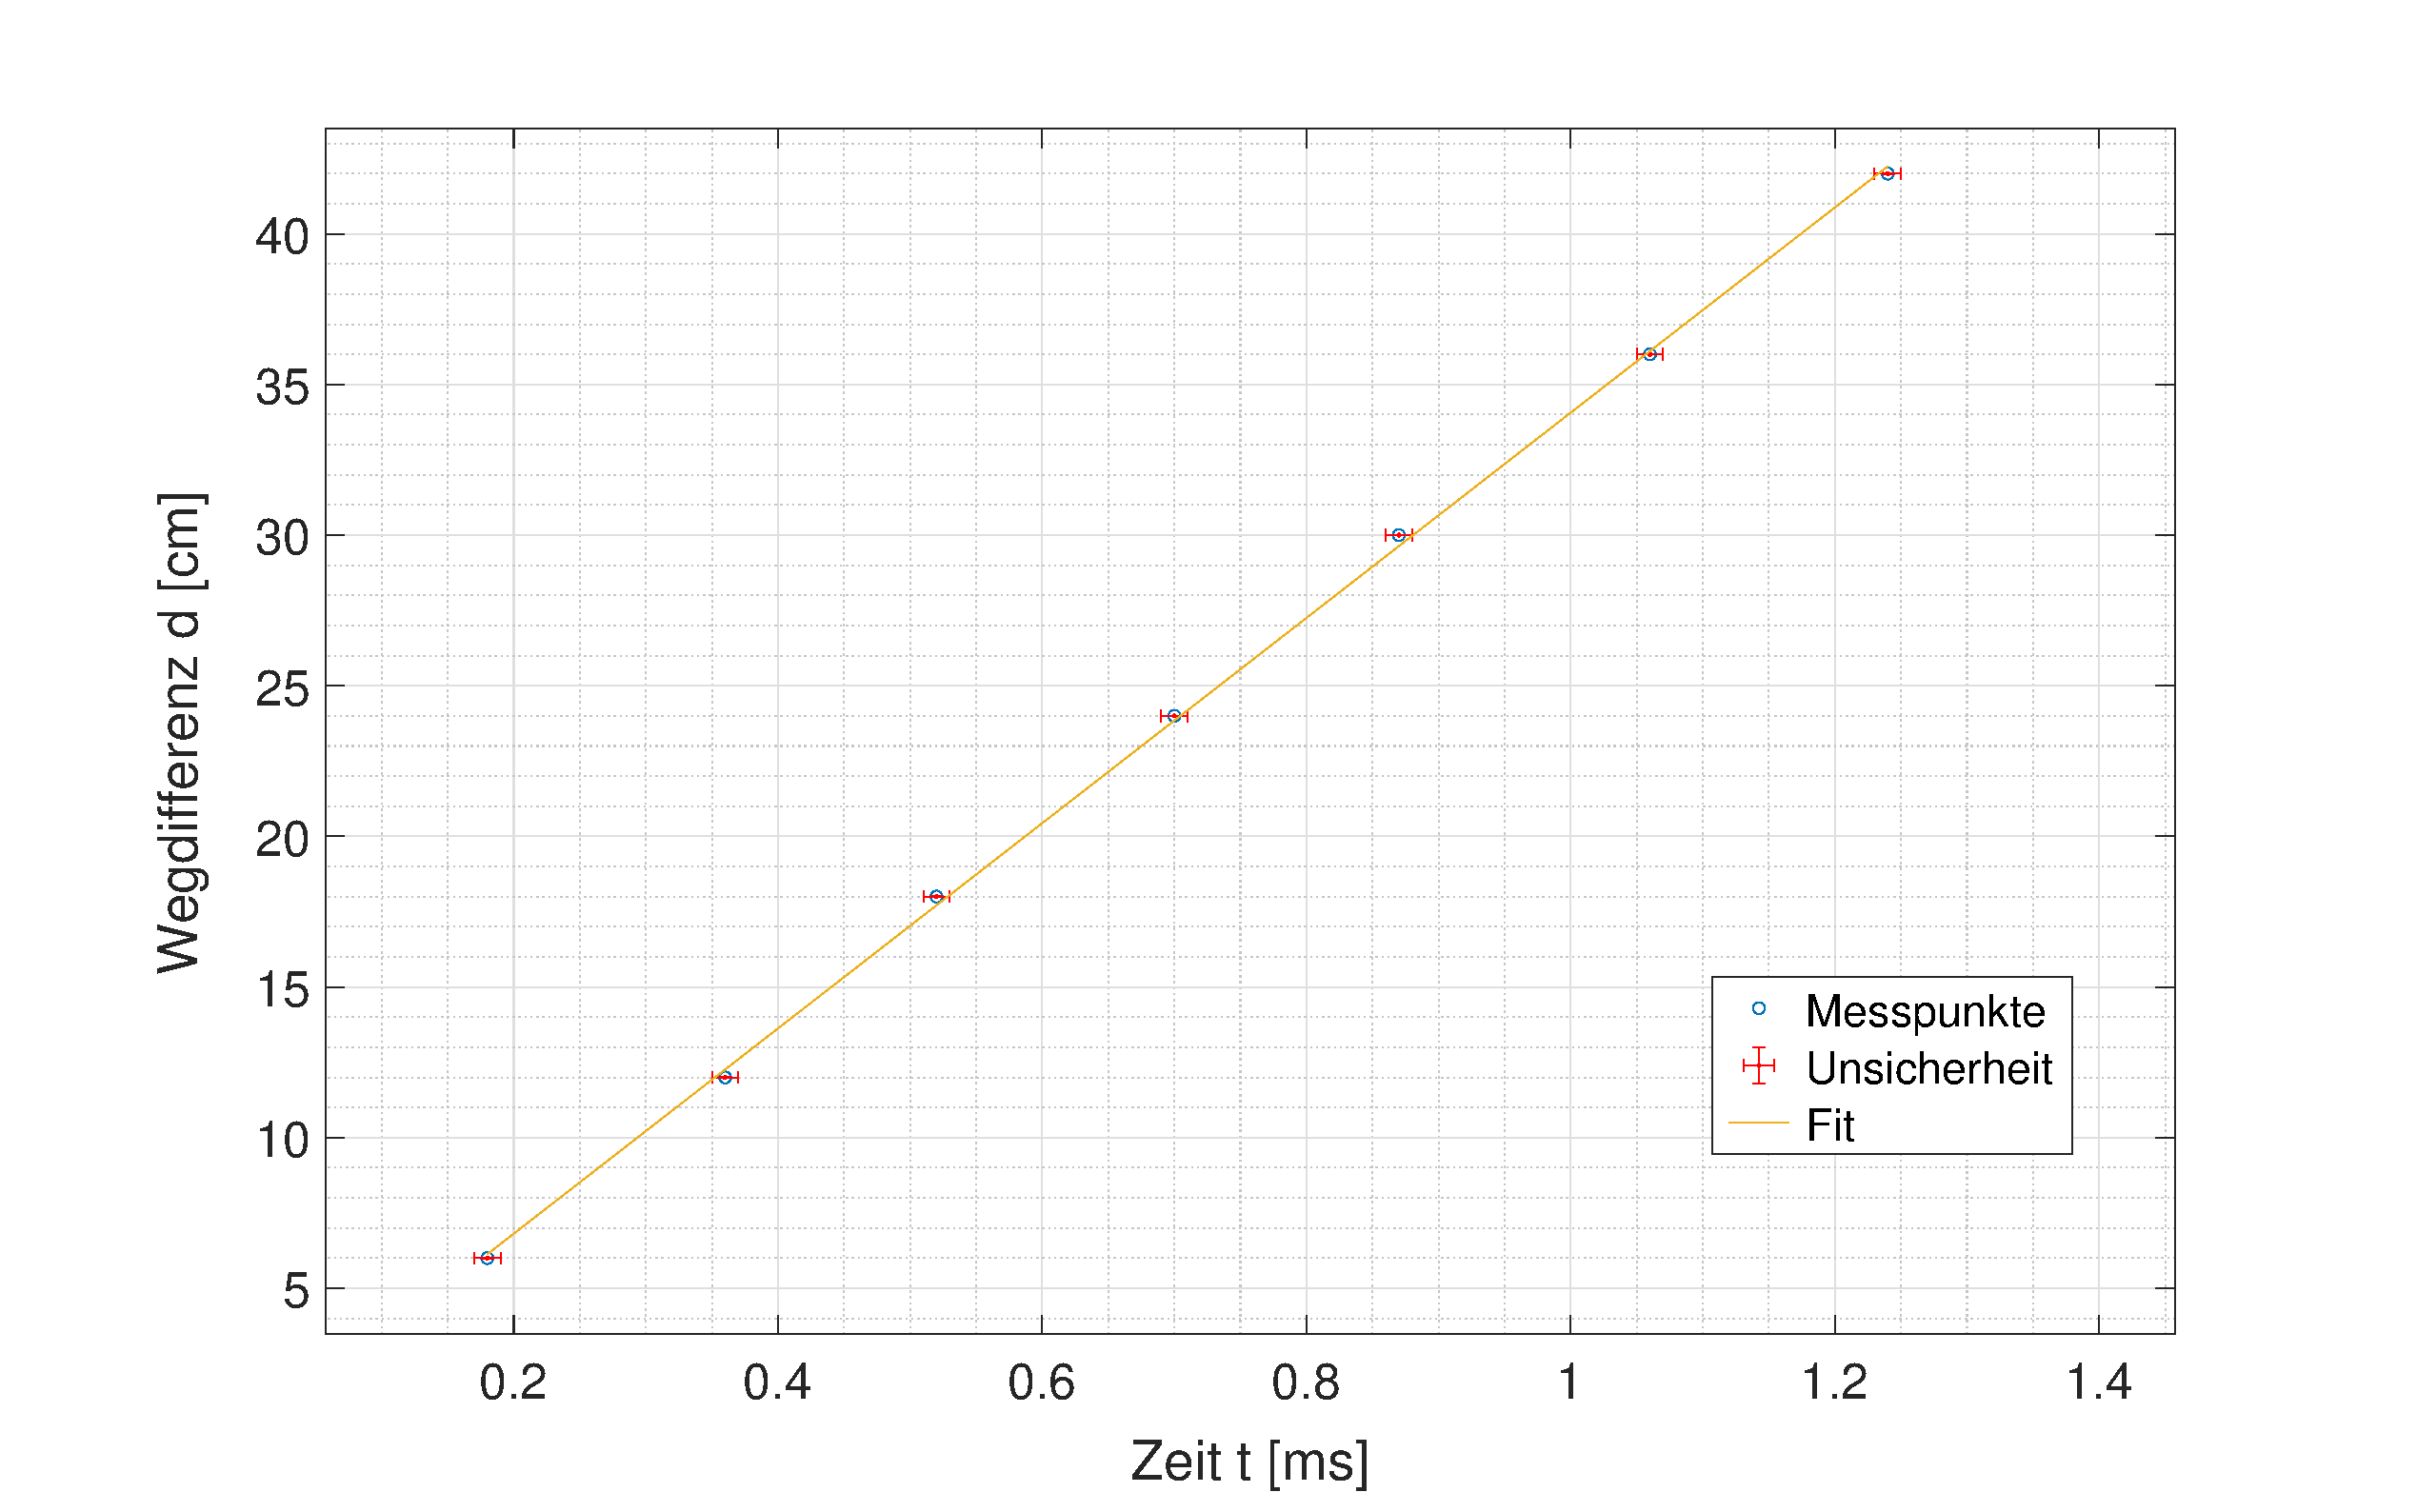
\includegraphics[scale=0.38]{laufzeit_luft.eps}
\caption{Laufzeitmessung in der Luft, Messpunkte mit Unsicherheit und Fitgerade.}
\end{figure}

Nun wird der Adiabatenkoeffizient $\kappa$ bestimmt. Dazu wird Gleichung 6 in Gleichung 7 eingesetzt und umgestellt zu:
\begin{equation}
\kappa = v^2 \cdot \frac{\rho_0}{p_0}\cdot \frac{T_0}{T}
\end{equation}
Mit $T=20\pm 2$ °C, $\rho_0 = 1,293$ \textrm{mg/cm$^3$} \cite{1}  \textrm{ und } $p_0=1013$ hPa \cite{1} erhält man $\kappa = 1,38 \pm 0,08$.
Der ermittelte Adiabatenkoeffizient stimmt innerhalb der Unsicherheiten mit dem Literaturwert von $1,4$ \cite{4} überein.
\subsection{Fehlerrechnung}
Ähnlich wie bei der Fehlerrechnung zu den Festkörpern, gibt es in diesem Teilversuch eine Unsicherheit für die Zeit $t$, welche durch die Ungenauigkeit des Oszilloskop Cursors kommt und eine Messunsicherheit bei der Abstandsmessung $d$. Die Ablesegenauigkeit des Oszilloskops ist diesmal $\SI{10}{\micro\meter}$ und bei der Messlatte nahmen wir $1$ mm an. \\
Mittels Gaußscher Fehlerfortpflanzung kommen wir schließlich auf eine Unsicherheit für die Schallgeschwindigkeit:
\begin{equation}
    u(v_i) = v_i \cdot \sqrt{\bigg(\frac{u(l)}{l}\bigg)^2 + \bigg(\frac{u(t)}{t}\bigg)^2},
\end{equation}
und den Adiabatenkoeffizient 
\begin{equation}
    u(\kappa) = \kappa \cdot \sqrt{\bigg(\frac{u(v)}{v}\bigg)^2 + \bigg(\frac{u(T)}{T}\bigg)^2}.
\end{equation}
\section{Stehende Wellen im Rohr}
\subsection{Versuchaufbau}
In diesem Teilversuch wird die Schallgeschwindigkeit in der Luft über die Wellenlänge einer stehenden Welle in einem halboffenen Rohr gemessen.
Ein Lautsprecher befindet sich am offenen Ende des Rohres.
Die Länge des Rohres kann durch das Verschieben eines Stempels variiert werden. 
Durch das Messen der Amplitude der Schallwellen am Eingang des Rohres kann festgestellt werden, bei welchen Längen des Rohres die am geschlossenen Ende des Rohres reflektierten Schallwellen maximal konstruktiv mit den neu erzeugten Schallwellen interferieren. 
Durch das variieren der Rohrlänge bestimmt man zunächst alle Amplitudenmaxima.
Mit konstanter, harmonischer Schwingung und bekannter Frequenz kann aus den Abständen der reflektierenden Rückseite zum Eingang des Rohres während der Amplitudenmaxima die Schallgeschwindigkeit bestimmt werden.

\begin{figure}[hbt!]
\centering
\includegraphics[scale=0.22]{aufbau_stehendewelle.png}
\caption{Aufbau Teilversuch Stehende Welle im Rohr \cite{1}.}
\end{figure}
\subsection{Auswertung}
Um eine gemittelte Distanz $\widetilde{d}$ zwischen den Amplitudenmaxima zu bestimmen, tragen wir zunächst die Länge $l$ vom Eingang des Rohres bis zum reflektierenden Ende gegen die Ordnung $n$ des Maximums auf. Der resultierende Graph ist in Abb. 7 zu sehen. Die Änderung $s$
\begin{equation}
s = d_{n+1} - d_{n}
\end{equation}
ist die Distanz, um die der Stempel verschoben werden muss, um von einem Maximum zum nächsten zu gelangen. Im Optimalfall gilt für die Distanzen $d_n$ des $n$-ten Maximums
\begin{equation}
d_n = s \cdot n + r
\end{equation}
was einer Geraden mit Steigung $s$ und y-Offset $r$ entspricht.
Um also die gemittelte Distanz $\widetilde{d}$ zwischen zwei Maxima aus Abb. 7 zu bestimmen, legen wir eine Ausgleichsgerade durch alle Messpunkte und betrachten ihre Steigung.
\begin{figure}[hbt!]
\centering
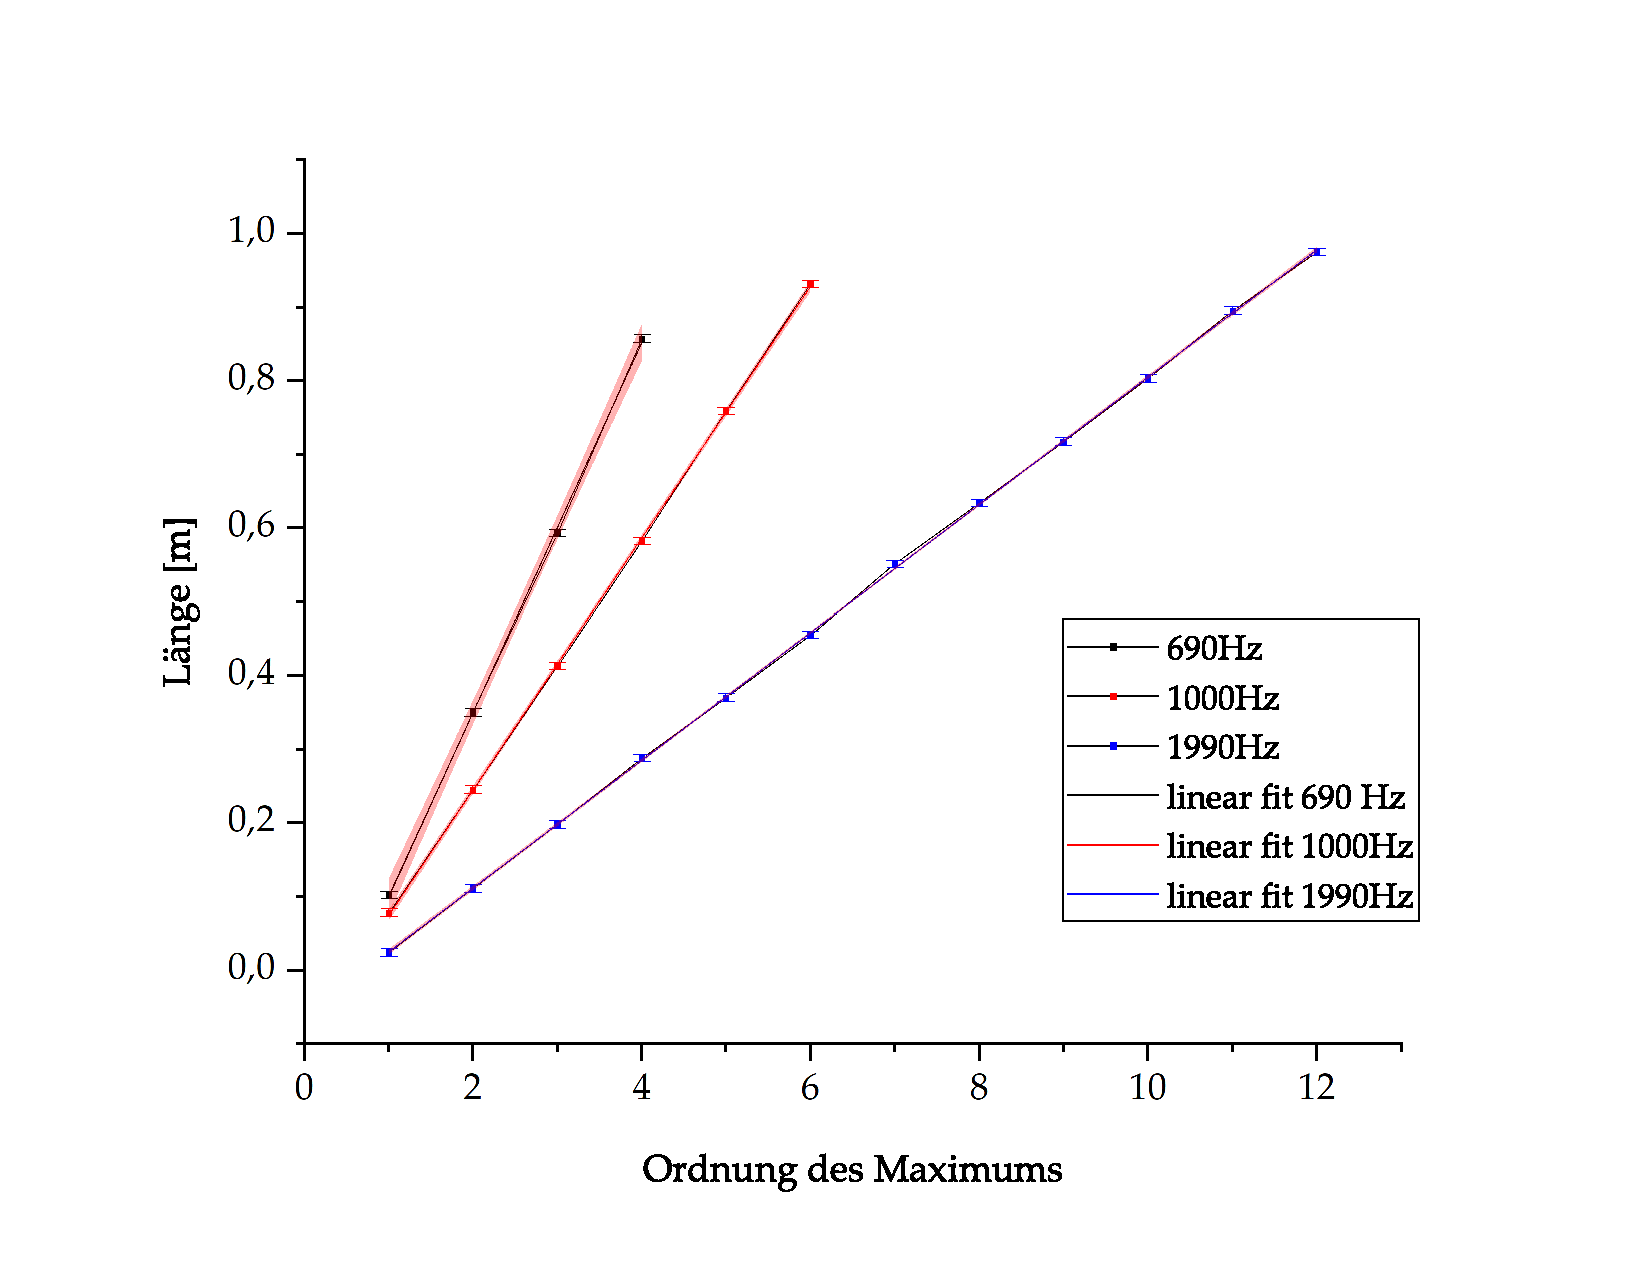
\includegraphics[width = 400pt]{length-vs-order.eps}
\caption{Distanz der Amplitudenmaxima gegen Ordnung mit Ausgleichsgerade und zugehörigem 95\%-Konfidenzintervall in rot}
\end{figure}
Es ergeben sich folgende Steigungen:

\begin{center}
\begin{tabular}{|c|c|}
\hline 
Frequenz & Steigung \\ 
\hline 
690(1)Hz & 0,2508(0,0031)m \\ 
\hline 
1000(1)Hz & 0,1704(0,0009)m \\ 
\hline 
1990(1)Hz & 0,0866(0,0003)m \\ 
\hline 
\end{tabular} 
\end{center}

Nimmt man an, dass am Eingang, Abb. 8 a), des einseitig geöffneten Rohres ein Amplitudenmaximum anliegt, lässt sich die Distanz $d_n$ vereinfacht schreiben als
\begin{equation}
d_n = \widetilde{d} \cdot n
\end{equation}
\begin{figure}[hbt!]
\centering
\includegraphics[width = 250pt]{WellenRohr.png}
\caption{Entwicklung einer Welle im einseitig geschlossenen Rohr}
\end{figure}
Zusammen mit der Beobachtung, dass das erste Maximum in diesem Fall, wie in Abb. 8 veranschaulicht, bei $\frac{\lambda}{2}$ b) auftritt, lässt sich $d_1$ als
\begin{equation}
d_1 = \widetilde{d} = \frac{\lambda}{2}
\end{equation}
schreiben. Somit folgt für $\lambda$
\begin{equation}
\lambda = 2 \cdot \widetilde{d}
\end{equation}
wie in Abb. 8 als c) dargestellt und für die Geschwindigkeit $v$
\begin{equation}
v = 2 \cdot f \cdot \widetilde{d}
\end{equation}

\begin{center}
\begin{tabular}{|c|c|}
\hline 
Frequenz & Geschwindigkeit \\ 
\hline 
690(1)Hz & 346,10(2,19)m/s \\ 
\hline 
1000(1)Hz & 341,49(1,45)m/s \\ 
\hline 
1990(1)Hz & 344,91(1,09)m/s \\ 
\hline 
\end{tabular} 
\end{center}
Der gewichtete Mittelwert ergibt eine Schallgeschwindigkeit von 344,08(1,35)m/s. 344,08m/s weicht von einem Literaturwert \cite{2} von 346m/s um 0,6$\%$ ab. Der Literaturwert verweist auf eine Temperatur von 25°C. Dies weicht vermutlich nach oben von der Temperatur während des Versuchs, die nicht dokumentiert wurde, ab.
Verglichen mit dem Wert $340,46(19,76)$ m/s aus Abschnitt 3.2 liegen beide Ergebnisse nahe beisammen und der Literaturwert unter Berücksichtigung der Temperatur innerhalb der Unsicherheiten. 

\subsection{Fehlerrechnung}

Der Eingangswert Länge $l$ hat zwei Messungsbedingte Unsicherheiten: beim Einstellen des Maximums von geschätzt $\pm$5mm und beim Ablesen der Skala von $\pm$1mm. Diese können einfach in eine Unsicherheit zusammengefasst werden mit
\begin{equation}
u_{Laenge} = \sqrt{5\textrm{mm}^2 + 1\textrm{mm}^2}
\end{equation}

Dieser Wert kann als y-Unsicherheit zum zeichnen der Abb. 7 als auch für die Ausgleichsgerade verwendet werden. Für die Steigung besagter Gerade gibt das Programm Origin eine Standardabweichung zurück. 

\begin{center}
\begin{tabular}{|c|c|}
\hline 
Frequenz & Standardabweichung \\ 
\hline 
690(1)Hz & 3,127mm \\ 
\hline 
1000(1)Hz & 0,876mm \\ 
\hline 
1990(1)Hz & 0,256mm \\ 
\hline 
\end{tabular} 
\end{center}

Diese Abweichung ist kleiner als die anfängliche Unsicherheit. Dies liegt möglicherweise daran, dass die Wahrscheinlichkeit, innerhalb einer Standardabweichung zu liegen, durch Datenpunkte, von denen keiner weit von der Ausgleichsgerade abweicht, ansteigt.

Für die Bestimmung der Geschwindigkeit mittels 
\begin{equation}
v = 2 \cdot f \cdot \widetilde{d}
\end{equation}
müssen wir diese Unsicherheit der Steigung mit der Unsicherheit der Frequenz verrechnen. 
Der Frequenzgenerator hat eine Unsicherheit von $1$ digit, was bei einer Einstellmöglichkeit von $4$ digits für alle verwendeten Frequenzen einer Unsicherheit von 1Hz entspricht.
Somit erhält man mit
\begin{equation}
u(v) = \sqrt{\frac{\delta v}{\delta f}^2 \cdot u(f)^2 + \frac{\delta v}{\delta\widetilde{d}}^2 \cdot u(\widetilde{d})^2} = \sqrt{\frac{\delta (2 \cdot f \cdot \widetilde{d})}{\delta f}^2 \cdot u(f)^2 + \frac{\delta (2 \cdot f \cdot \widetilde{d})}{\delta\widetilde{d}}^2 \cdot u(\widetilde{d})^2}
\end{equation}
Werte von
\begin{center}
\begin{tabular}{|c|c|}
\hline 
Frequenz & Unsicherheit der Geschwindigkeit \\ 
\hline 
690(1)Hz & 2,19m/s \\ 
\hline 
1000(1)Hz & 1,45m/s \\ 
\hline 
1990(1)Hz & 1,09m/s \\ 
\hline 
\end{tabular} 
\end{center}
und schließlich mit dem gewichteten Mittelwert
\begin{equation}
v_{Mittelwert} = \frac{\frac{1}{u_{690}^2} \cdot v_{690} + \frac{1}{u_{1000}^2} \cdot v_{1000} + \frac{1}{u_{1990}^2} \cdot v_{1990}}{\frac{1}{u_{690}^2} + \frac{1}{u_{1000}^2} + \frac{1}{u_{1990}^2}}
\end{equation}
den oben genannten Wert für die Schallgeschwindigkeit.

Für die Unsicherheit dieser Geschwindigkeit müssen die äußere und innere Unsicherheit betrachtet werden:
\begin{equation}
u(v_{Mittelwert}) = max(u_{int}, u_{ext}).
\end{equation}
Die innere Unsicherheit lässt sich bestimmen mit:
\begin{equation}
u_{int}(v) = \sqrt{\frac{1}{\frac{1}{u_{690}^2} + \frac{1}{u_{1000}^2} + \frac{1}{u_{1990}^2}}}
\end{equation}
Für die äußere Unsicherheit gilt:
\begin{equation}
u_{ext} = \sqrt{\frac{\frac{1}{u_{690}^2}\cdot(v_{Mittelwert} - v_{690})^2+ \frac{1}{u_{1000}^2}\cdot(v_{Mittelwert} - v_{1000})^2 + \frac{1}{u_{1990}^2}\cdot(v_{Mittelwert} - v_{1990})^2}{(3-1)\cdot (\frac{1}{u_{690}^2} + \frac{1}{u_{1000}^2} + \frac{1}{u_{1990}^2})}}
\end{equation}

\section{Literaturverzeichnis}
\begin{thebibliography}{9}
\bibitem{1}
Fakultät für Physik. \emph{Akustik} (AKU. Technische Universität München. 30.05.2022.
\textbf{URL:} \url{https://www.ph.tum.de/academics/org/labs/ap/ap1/AKU.pdf}

\bibitem{2}
W.M.Haynes, Hrsg. \emph{CRC Handbook of Chemistry and Physics} (CRC Press, 04.06.2014)

\bibitem{3}
F. Kohlrausch, \emph{Praktische Physik Band 3} (B. G. Teubner Stuttgart, 24. Auflage, 1996)

\bibitem{4}
\emph{Table of Thermal Properties of Gases.} (National Bureau of Standards Circular 564 (1955)

\bibitem{5}
Volker Läpple \emph{Einführung in die Festigkeitslehre: Lehr- und Übungsbuch} (Vieweg Verlag, 2011)

\end{thebibliography}
\section{Anhang}
\subsection{Laborbuch}
\includepdf[pages=-]{Protokoll.pdf}
\end{document}
